\documentclass[a4paper,11pt,twocolumn]{article}

\usepackage{lrec2014}

\usepackage{polyglossia}
\setdefaultlanguage[variant=australian]{english}

\usepackage{fontspec}
\usepackage{xunicode}
\usepackage{xltxtra}
\usepackage{natbib}
\usepackage{multirow}
%\usepackage{fullpage}
\usepackage{multirow}
\usepackage[colorlinks=true,citecolor=black,linkcolor=black,urlcolor=blue]{hyperref}
\usepackage[small,bf]{caption}
\usepackage{booktabs}
\usepackage{jnwmaps}

\defaultfontfeatures{Mapping=tex-text}
\setromanfont{Times New Roman}
\newfontfamily\symbl[Scale=MatchLowercase]{FreeSerif}
\newfontfeature{IPA}{+mgrk}
\newfontfamily\qipa[IPA,Scale=MatchLowercase]{FreeSerif}

\newcommand{\tags}[1]{\texttt{#1}}

\bibdata{kipchak-paper}


\title{Finite-state morphological transducers for three Kypchak languages}

%\author{Jonathan North Washington \\
%Departments of Linguistics and Central Eurasian Studies\\
%Indiana University\\
%Bloomington, IN 47405 (USA)\\
%\texttt{jonwashi@indiana.edu} \and
%Ilnar Salimzyanov  \\
%Kazan Federal University \\
%Kazan, Republic of Tatarstan\\
%(Russian Federation) \\
%\texttt{ilnar.salimzyan@gmail.com} \and 
%Francis M. Tyers\\
%5HSL-fakultehta, \\
%UiT Norgga árktalaš universitehta, \\
%9019 Romsa (Norway)\\
%\texttt{francis.tyers@uit.no} 
%}

%FIXME: usually star comes first, then daggers
\name{Jonathan North Washington$^\dagger$, Ilnar Salimzyanov$^\ddagger$, Francis M. Tyers$^\star$}

\address{$^\dagger$Departments of Linguistics and Central Eurasian Studies\\
Indiana University\\
Bloomington, IN 47405 (USA)\\
\texttt{jonwashi@indiana.edu} \and
$^\ddagger$Institut für Maschinelle Sprachverarbeitung \\
Universität Stuttgart\\
Stuttgart (Germany) \\
\texttt{ilnar@ilnar} \and 
$^\star$HSL-fakultehta \\  
UiT Norgga árktalaš universitehta \\
9019 Romsa (Norway)\\
\texttt{francis.tyers@uit.no} 
}

\abstract{This paper describes the development of free/open-source finite-state morphological transducers for three Turkic languages---Kazakh, Tatar, and Kumyk---representing one language from each of the three sub-branches of the Kypchak branch of Turkic.  The finite-state toolkit used for the work is the Helsinki Finite-State Toolkit (HFST).  This paper describes how the development of a transducer for each subsequent language took less development time.  An evaluation is presented which shows that the transducers all have a reasonable coverage---around 90\%---on freely available corpora of the languages, and high precision over a manually verified test set. \\
	\Keywords{Kazakh, Tatar, Kumyk, morphology, transducer}
}

\begin{document}

\maketitleabstract{}

\section{Introduction}

This paper describes the development of free/open-source morphological transducers for three closly related languages: Kazakh, Tatar, and Kumyk.  Morphological transducers are computational models of the languages' morphology, and are used to output morphological analyses from word forms and vice-versa.

These transducers were all developed as part of the Apertium project, which is aimed at creating rule-based MT systems for lesser resourced languages.  As such, the transducers were developed with the intent that they be used as morphological analysers and generators in RBMT systems.  However, this sort of finite-state transducer has a wide variety of usages, including for creating proofing tools such as spellcheckers and grammarcheckers.

%the potential uses of morphological transducers is much broader; for example, we have found that they are easily converted to spell checkers.

All three transducers were designed as ``ports'' of Apertium's Kyrgyz morphological transducer \citep{washington2012}.  The Tatar and Kazakh transducers are used in a release-quality Kazakh-Tatar MT system \citep{salimzyanov2013}.

%FIXME: brief background on how, when, and with what support were developed?
% In Apertium project, Turkic transducers were developed either as part of Turkic-to-Turkic machine translators, or they started as a "port" (in particular of morphotactics) of already existing Turkic transducers.

%The transducers for these languages

% FIXME: what are transducers used for ?

This paper overviews the languages (§\ref{sec:lgs}), provides background on these morphological transducers and related previous work (§\ref{sec:bg}), describes the development effort and contents of the transducers (§\ref{sec:methodology}), evaluates the effectiveness of these transducers (§\ref{sec:evaluation}), and summarises the findings (§\ref{sec:conclusions}).

\section{Languages}\label{sec:lgs}

The three languages for which transducers were developed belong to the Northwestern branch of the Turkic family, which is often referred to as the Kypchak branch.  This branch can be divided into three subbranches.  Kumyk is a member of the Western Kypchak group, Tatar is a member of the Northern Kypchak group, and Kazakh is a member of the Southern Kypchak group \citep[82-83]{histofturkic}.\footnote{It is the belief of the authors of this paper that Kyrgyz constitutes a fourth branch.}  As such, each of these three languages represents one of the three branches of Kypchak.  The geographic distribution of the languages is shown in map \ref{map1}.

\begin{map*}[htbp]
	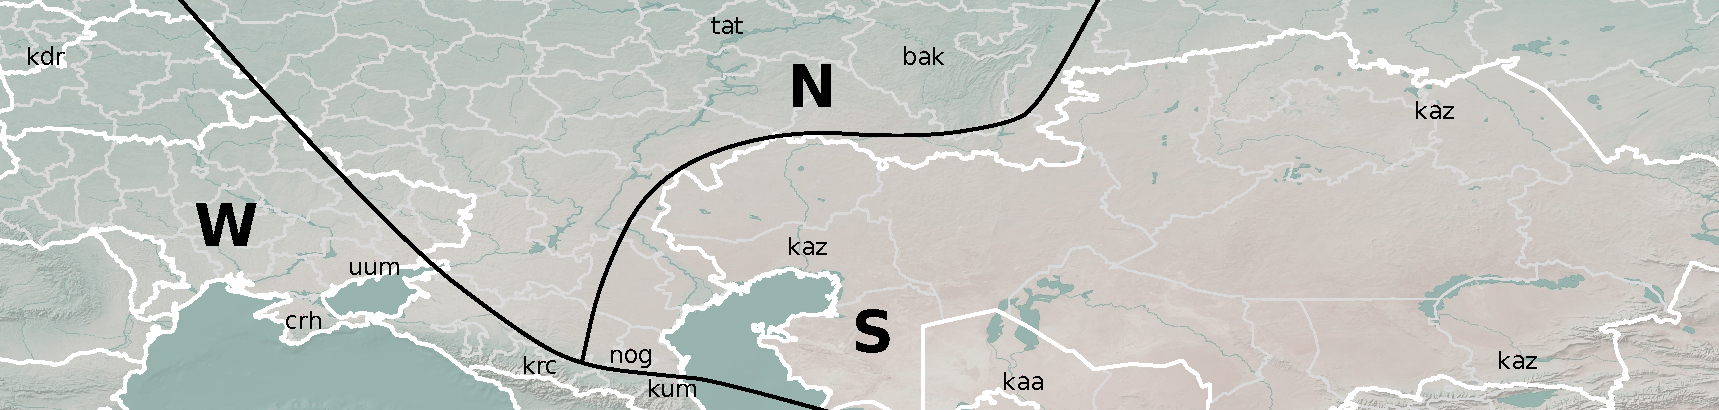
\includegraphics[width=\textwidth]{map/map}
	\caption{The three sub-branches of Kypchak (North, South, West), roughly divided with black lines, showing the geographic distribution of the three languages for which transducers were developed: Tatar (\texttt{tat}), Kazakh (\texttt{kaz}), and Kumyk (\texttt{kum}).}
	\label{map1}
\end{map*}

These languages have different amounts of linguistic influence from other Turkic branches (e.g., moderate Oghuz (SE) influence in the Western group, slight Oghuz influence in the Northern group) and from Mongolic languages (moderate influence on the Southern group, lighter in the other groups), and all have heavy influence from Persian.

\subsection{Kazakh}
Kazakh /q{\symbl ɑ}z{\symbl ɑ}q/ is spoken primarily in Kazakhstan, where it is the national language, where it is co-official with Russian.  Large communities of native speakers also exist in China, neighbouring Central-Eurasian republics, and Mongolia. Ethnologue estimates
the total number of speakers to be around 8 million \citep{ethnologue}.

%Estimates of the total number of speakers range from 8 million \citep{ethnologue} to 11 million \citep{nationalencyklopedin} people.

\subsection{Tatar}
Tatar /t{\symbl ɒ}t{\symbl ɑ}r/ is spoken in and around Tatarstan, by approximately 5.4 million people \citep{ethnologue}.  It is co-official with Russian in Tatarstan --- a republic of the Russian Federation.  A majority of native speakers of both languages are bilingual in Russian. %, and the standard varieties our system FIXMEs are written in Cyrillic.

\subsection{Kumyk}
Kumyk /qumuq/ is spoken in Dagestan, a republic of the Russian Federation, where it is co-official with a number of other national languages \citep{ethnologue}.  There are approximately 430 thousand speakers \citep{ethnologue}.

\section{Background}\label{sec:bg}
\subsection{Morphological transducers, previous work}
%FIXME: need a source, maybe something by Tommi?
The objective of a morphological transducer is twofold: firstly to take surface forms (e.g., алдым) and generate all possible lexical forms, and secondly to take lexical forms (e.g.,  ал{\tt {\small <v><tv><ifi><p1><sg>}}, алд{\tt {\small <n><px1sg><nom>}},\footnote{For a description of the tags used throughout this paper, please see Appendix~\ref{app:glossary}.} etc.) and generate one or more surface forms.  As they are implemented as finite-state transducers, they are reversible by default. For more information on usin finite-state transducers for morphological analysis and generation, the reader is referred to \cite{beesley2003}.

The transducers were designed based on the Helsinki Finite State Toolkit \citep{hfst/2011} which is a free/open-source reimplementation of the Xerox finite-state toolchain, popular in the field of morphological analysis.  It implements both the \textbf{lexc} formalism for defining lexicons, and the \textbf{twol} and \textbf{xfst} formalisms for modeling morphophonological rules.  It also supports other finite state transducer formalisms such as \textbf{sfst}.  This toolkit has been chosen as it -- or the equivalent XFST -- has been widely used for other Turkic languages, such as Turkish \citep{coltekin2010}, Crimean~Tatar~\citep{altintas2001}, Turkmen \citep{tantug2006}, and Kyrgyz \citep{washington2012}, and is available under a free/open-source licence.

The authors learnt of another Kazakh morphological transducer in existence \citep{bekmanova2013} only after this paper was submitted and our transducer was released.  We have not yet been able to evaluate this system or compare it to ours.

Creating morphological transducers in the above-mentioned formalisms involves encoding linguistic knowledge about the language in the formalisms.  The lexc and twol formalisms resemble linguistic formalisms, allowing the coders to work with abstractions resembling linguistic categories such lexemes, morphemes, phonemes, and even archiphonemes.

\subsection{Description}

%FIXME: keep revision number up to date
The transducers are available / under development in apertium's subversion repository,\footnote{\url{https://svn.code.sf.net/p/apertium/svn/languages/}} in the directories apertium-kaz, apertium-tat, and apertium-kum.  The revision of the entire subversion repository that the numbers (stem counts, evaluation, etc.) in this paper represent is \texttt{r48137}.


\section{Methodology}\label{sec:methodology}
% cite Hengeveld (1992) ?

% Noun morphotactics -- is basically equivalent in all three, except for archiphonemes
% Adjective categorisation
% Adverb categorisation
% "Irregular" harmony, caused by orthography
% Non-finite verb form categorisation "converbs"

% Handling numerals and acronyms.

% Russian loans not obeying phonology N5, e.g. ё vs . самолёт


\subsection{Development effort}

The three transducers discussed in this paper are for Kazakh, Tatar, and Kumyk.  The Kazakh and Tatar transducers were originally created as part of an experimental Kazakh-Tatar machine translation system in December of 2010.  The Kazakh transducer was expanded during Google Code-In 2010 and 2011, and the Tatar transducer was expanded as part of a prototype Tatar and Bashkir machine translation system \citep{tyerswashingtonsalimzyanbattalov12}.  The Kazakh-Tatar machine translation system, along with the two transducers, was expanded to production-level quality as part of a Google Summer of Code project in 2012 \citep{salimzyanov2013}.

The Kumyk transducer was developed starting at the beginning of October, 2013 as experiment to see how difficult it would be to extend lessons learned from the development of the Tatar and Kazakh transducers to a related language.  While the Kazakh and Tatar transducers took around six months work to reach their current coverage level, the Kumyk transducer only took a couple weeks to reach this level of quality (see Figure~\ref{fig:kumcov}).  This paper explores how the development of the Kumyk transducer benefitted from knowledge gained from the development of the Tatar and Kazakh transducers.

The morphotactics\footnote{The morphotactics of a language is the way in which morphemes can be combined to create words.} of Turkic languages are complex enough that even a linguist who is fluent in the language and has a good linguistic understanding of it may not understand how exactly all morphemes combine.  Native speakers educated about the morphology of their languages also do not have an explicit knowledge of the complete morphotactics.  Hence it often becomes necessary to use fieldwork methodology to elicit the full extent of the morphotactics, be this a linguist with little to no knowledge of a Turkic language working with a native speaker, or a native speaker who understands the extent of what knowledge is necessary to encode in the transducer.  When there is no native speaker of a particular language available, the authors have found that information previously encoded about a closely related language or the intuitions of a speaker of a closely related language may be combined with the use of textual corpora to ``elicit'' information about the morphotactics of a language.  Depending on the contents of corpus and chance, this may not result in a completely accurate model, but it is possible to be thorough.

The Kazakh morphotactics were originally developed based on the Kyrgyz transducer, which was co-authored by the first author, who is fluent in and has a good linguistic knowledge of Kyrgyz and two native speakers of Kyrgyz. The first author also developed the Kazakh morphotactics who is fluent in and has a good linguistic understanding Kazakh.  The morphotactics of Tatar were developed for the most part by the third author, a native speaker of Tatar, who also worked to polish off the morphotactics of the Kazakh transducer.

%As the authors found it difficult to locate native speakers of Kumyk, the morphotactics of the Kumyk transducer were developed based on the existing encoded morphotactics of Kazakh and Tatar (and occasionally Kyrgyz), with consultation of corpora, as described above.  A dictionary \citep{bammatov1960} and a grammar \citep{olmesov2000} of Kumyk were also consulted as needed. 

In order to create the Kumyk transducer, we approached one of the major parts of speech at a time. We started with the nouns, copying the 
continuation lexica\footnote{A continuation lexicon is a set of morphemes, for example, in the Turkic languages there is a continuation lexicon for `case' which includes the possible case suffixes.} (nominal morphotactics) from the Kazakh transducer. The suffixes were then replaced with the Kumyk suffixes according to the grammar \citep{olmesov2000}. Where the grammar was not explicit regarding a suffix form, we looked the corpus for possible forms and at their contexts. The same process was done for verbs. 

% FIXME: how long it took
% FIXME: make a graph for the kumyk one

\begin{figure}
%\centering
\hspace{-15pt}
    \rotatebox{-90}{
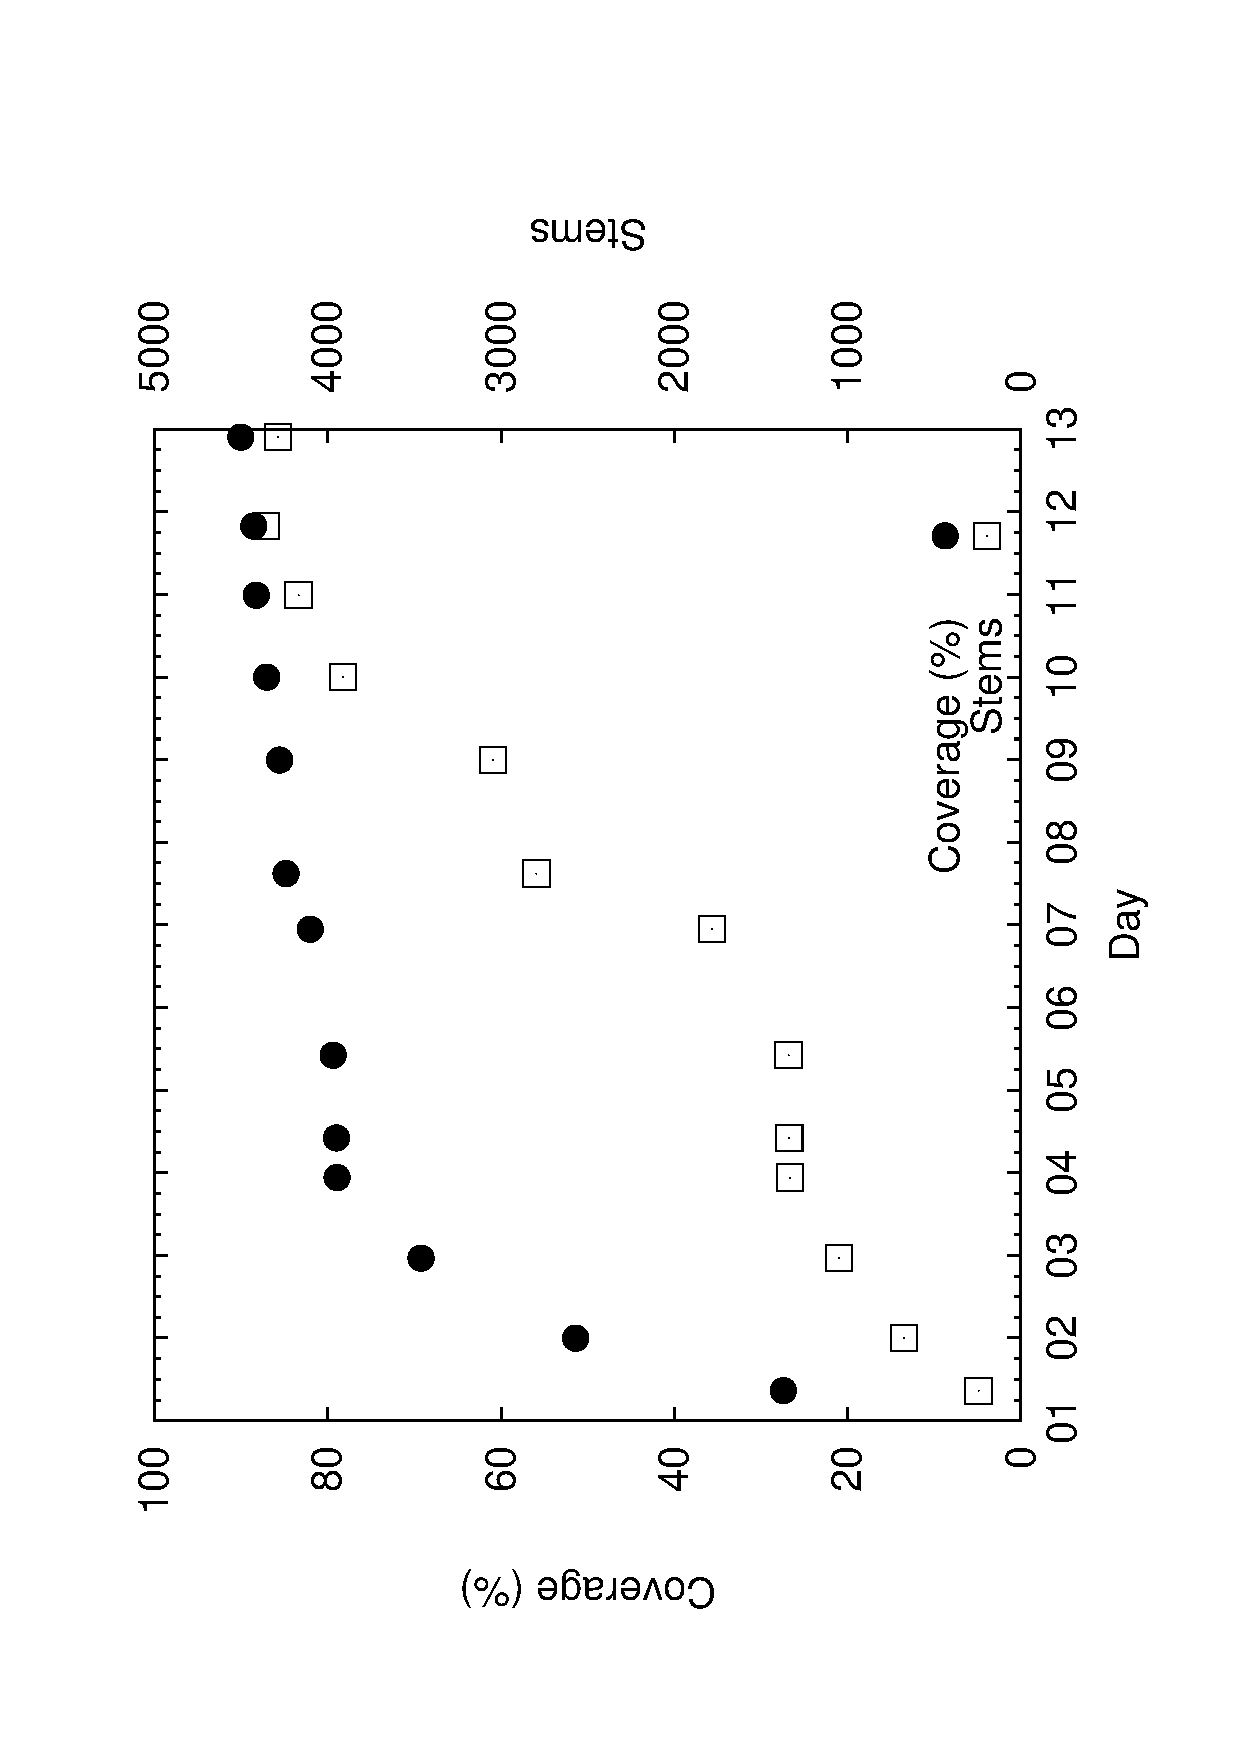
\includegraphics[width=0.4\textwidth]{graphs/kumyk-yoldash-coverage}
}

\caption{Number of stems and coverage of corpus over time. Time is measured in days 
starting from the 2nd October 2013. The graph shows that to reach 80\% coverage, took
around a week, and to reach 90\% took another week.}
\label{fig:kumcov}
\end{figure}

\subsection{Transducer contents}

Each transducer's lexc source consists of lists of stems, with each stem pointing at a complex continuation lexicon containing the appropriate morphology for the type of stem.  

%FIXME: update for the three languages
The tagset for each transducer is designed to be compatible with the others.  Each transducer consists of about 120 separate tags, of which close to 20 cover the main parts of speech (noun, verb, adjective, adverb, postposition, interjection, etc.).  The remaining tags cover morphological subcategorisation for e.g.\ case, number, person, possession, transitivity, tense-aspect-mood, etc.  The tags are represented as multicharacter symbols, between less-than \texttt{<} and greater-than \texttt{>} symbols.  The tagset is quite extensive and still not entirely stabilised, so a full listing is not included here.  However, the tags are listed in the source code of the transducers, along with comments describing their usage.

%\subsection{Statistics}

Table \ref{table:stems} lists the number of stems of the primary categories in each transducer.

\begin{table}
\begin{center}
\begin{tabular}{lrrr}
		\toprule
\multirow{2}{*}{\textbf{Part of speech}} & \multicolumn{3}{c}{\textbf{Number of stems}} \\ \cline{2-4}
                        & Kazakh & Tatar & Kumyk \\
		\midrule
		Noun & 2463 & 2692 & 2588 \\
		Verb & 1587 & 1333 & 262 \\
		Adjective & 823 & 852 & 217 \\
		Proper noun & 5412 & 3523 & 1444 \\
		Adverb & 197 & 205 & 63 \\
		Numeral & 63 & 67 & 45 \\
		Conjunction & 52 & 50 & 15 \\
		Postposition & 56 & 46 & 12 \\
		Pronoun & 17 & 17 & 18 \\
		Determiner & 42 & 37 & 9 \\
		\midrule
		Total: & 10942 & 9009 & 4687 \\
		\bottomrule
\end{tabular}
 \caption{Number of stems in each of the categories. The large number of noun stems as compared
    to other parts of speech in the Kumyk transducer can be explained by the relative ease of 
    categorising nouns as opposed to adjectives, adverbs and verbs. Adding a noun essentially involves
    choosing between loan word and native word. Where adding stems from the other main categories 
    requires more in depth categorisation.}
 \label{table:stems}
\end{center}

\end{table}

% FIXME: example output

\begin{table*}

% kaz: ^Құдай/Құдай<n><nom>/Құдай<n><attr>/Құдай<n><nom>+е<cop><p3><pl>/Құдай<n><nom>+е<cop><p3><sg>$ ^Өзінің/Өз<prn><ref><p3><sg><gen>$ ^жаратқандарының/жарат<v><tv><ger_past><pl><px3sp><gen>/жарат<v><tv><gpr_past><subst><pl><px3sp><gen>$ ^бәріне/бәрі<prn><qnt><px3sp><dat>$ ^қарап/қара<v><tv><prc_perf>/қара<v><tv><gna_perf>/қара<v><tv><prc_perf>$^,/,<cm>$ ^өте/өт<v><tv><prc_impf>/өте<adv>/өте<v><tv><imp><p2><sg>$ ^жақсы/жақсы<adj>/жақсы<adv>/жақсы<adj><advl>/жақсы<adj><subst><nom>/жақсы<adj>+е<cop><p3><pl>/жақсы<adj>+е<cop><p3><sg>/жақсы<adj><subst><nom>+е<cop><p3><pl>/жақсы<adj><subst><nom>+е<cop><p3><sg>$ ^екенін/е<cop><ger_past><px3sp><acc>$ ^көрді/көр<vaux><ifi><p3><pl>/көр<vaux><ifi><p3><sg>/көр<v><tv><ifi><p3><pl>/көр<v><tv><ifi><p3><sg>$^./.<sent>$ 
% tat: ^Аллаһ/Аллаһ<n><nom>/Аллаһ<n><attr>/Аллаһ<n><nom>+и<cop><p3><sg>$ ^Үзе/Үз<prn><ref><p3><sg><nom>/Үз<prn><ref><p3><sg><nom>+и<cop><p3><sg>$ ^яраткан/ярат<v><tv><gpr_past>/яраткан<adj>/ярат<v><tv><ger_past><nom>/яраткан<adj><advl>/ярат<v><tv><past><p3><sg>/ярат<v><tv><gpr_past><subst><nom>/яраткан<adj><subst><nom>/яраткан<adj>+и<cop><p3><sg>/яраткан<adj><subst><nom>+и<cop><p3><sg>$ ^нәрсәләргә/нәрсә<prn><itg><pl><dat>$ ^карап/кара<vaux><prc_perf>/кара<vaux><gna_perf>/кара<v><tv><prc_perf>/кара<v><tv><gna_perf>$^,/,<cm>$ ^аларның/ул<prn><dem><pl><gen>/алар<prn><pers><p3><pl><gen>$ ^бик/бик<adv>/бик<n><nom>/бик<n><attr>/бик<n><nom>+и<cop><p3><sg>$ ^яхшы/яхшы<ij>/яхшы<adj>/яхшы<adj><advl>/яхшы<adj><subst><nom>/яхшы<adj>+и<cop><p3><sg>/яхшы<adj><subst><nom>+и<cop><p3><sg>$ ^икәнен/и<cop><ger_past><px3sp><acc>$ ^күрде/күр<v><tv><ifi><p3><sg>$^./.<sent>$
% kum: ^Аллагь/аллагь<n><nom>/аллагь<n><attr>$ ^Оьзю/оьз<prn><ref><px3sp><nom>$ ^яратгъан/ярат<v><tv><gpr_past>/ярат<v><tv><gpr_past><subst><nom>/ярат<v><tv><ger_past><nom>/ярат<v><tv><past><p3><sg>$ ^затлагъа/зат<n><pl><dat>$ ^къарап/къара<v><tv><prc_perf>/къара<v><tv><gna_perf>$^,/,<cm>$ ^олар/о<prn><dem><pl><nom>/олар<prn><pers><p3><pl><nom>$ ^бек/бек<adv>$ ^яхшы/яхшы<adj>/яхшы<adj><subst><nom>$ ^экенин/э<cop><ger_past><px3sp><acc>$ ^гёрген/гёр<v><tv><gpr_past>/гёр<v><tv><gpr_past><subst><nom>/гёр<v><tv><ger_past><nom>/гёр<v><tv><past><p3><sg>$^../..<sent>$


%
%\textbf{Kazakh:} Құдай Өзінің жаратқандарының бәріне қарап, өте жақсы екенін көрді. \\
%% (close to kaz) Ходай Үзенең яратканнарының барысына карап, бик яхшы икәнен күрде. \\
%% (from the actual translation of the Bible) Аллаһ үзе яраткан нәрсәләрне күздән кичерде, һәм, менә, һәр нәрсәнең гаять яхшы икәнлеген күрде. \\
%\textbf{Tatar:} Аллаһ Үзе яраткан нәрсәләргә карап, аларның бик яхшы икәнен күрде. \\
%\textbf{Kumyk:} Аллагь Оьзю яратгъан затлагъа къарап, олар бек яхшы экенин гёрген. \\
%
\centering

\scalebox{0.81}{
\begin{tabular}{lll}
 \textbf{Kazakh} & \textbf{Tatar} & \textbf{Kumyk} \\
\hline
 Құдай Өзінің жаратқандарының  &  Аллаһ Үзе яраткан нәрсәләргә карап, & Аллагь Оьзю яратгъан затлагъа\\
 бәріне қарап, өте жақсы екенін көрді. &  аларның бик яхшы икәнен күрде. & къарап, олар бек яхшы экенин гёрген. \\
\hline
 Құдай\tags{<n><nom>} & Аллаһ\tags{<n><nom>} & Аллагь\tags{<n><nom>}  \\
 Өз\tags{<prn><ref><px3sp><gen>} & Үз\tags{<prn><ref><px3sp><nom>} & Оьз\tags{<prn><ref><px3sp><nom>} \\
 жарат\tags{<v><tv><ger\_past><pl><px3sp><gen>} & ярат\tags{<v><tv><gpr\_past>} & ярат\tags{<v><tv><gpr\_past>} \\
 бәрі\tags{<prn><qnt><px3sp><dat>} & нәрсә\tags{<prn><itg><pl><dat>} & зат\tags{<n><pl><dat>} \\
 қара\tags{<v><tv><gna\_perf>} & кара\tags{<v><tv><gna\_perf>} & къара\tags{<v><tv><gna\_perf>} \\ 
,\tags{<cm>} & ,\tags{<cm>} & ,\tags{<cm>} \\
 ---      & алар\tags{<prn><pers><p3><pl><gen>} & олар\tags{<prn><pers><p3><pl><nom>} \\
 өте\tags{<adv>} & бик\tags{<adv>} & бек\tags{<adv>} \\
 жақсы\tags{<adj>} & яхшы\tags{<adj>} & яхшы\tags{<adj>} \\
 е\tags{<cop><ger\_past><px3sp><acc>} & и\tags{<cop><ger\_past><px3sp><acc>} & э\tags{<cop><ger\_past><px3sp><acc>} \\
 көр\tags{<v><tv><ifi><p3><sg>} & күр\tags{<v><tv><past><p3><sg>} & гёр\tags{<v><tv><past><p3><sg>} \\  
 .\tags{<sent>} & .\tags{<sent>} & .\tags{<sent>} \\
\hline
\end{tabular}
}
\label{table:exoutput}
\caption{An example of the output of each of the morphological transducers for the same 
  sentence (``And God saw every thing that he had made, and, behold, it was 
  very good.'', Genesis 1:31). The sentence may be very roughly glossed as ``God own-his created things/everything-at looking,
  their very good being saw''. The output has been 
  abbreviated to only show the appropriate tag in context, 
  the actual output would be ambiguous. Refer to Appendix~\ref{app:glossary} for tag descriptions.}

\end{table*}

\subsection{Categorisation and tagset}

The open categories in Turkic languages can be broadly split into two groups: nominals
and verbals. The nominals group can be further split into nouns, adjectives and adverbs.
We define nouns as stems that can be subjects of a finite verb, adjectives as stems that principally qualify 
nouns, and adverbs as stems that principally modify verbs.

Most of the stems in the lexicon can be used, with no extra suffixes in any of these functions, for 
example the adjective жақсы in Kazakh can be used as attributively, жақсы кітап `good book', adverbially
жақсы ойнадыңыз `(you) played well', and substantively (as a noun) `жақсы келетін еді' `(the) good (ones) would come'. This
is a productive process and relevant to the morphotactics as an adjective used substantively may take the 
full range of case and possessive suffixes, and adjectives used adverbially will take a different set of 
clitics to adjectives used substantively and attributively. 

However, this is not completely productive. A grammar which allows all adjectives to function
as nouns and adverbs will overgenerate (and overanalyse). However, most grammars do not 
mention that there are exceptions to this productive process.

Other analysers for Turkic languages---such as \texttt{TRmorph} \citep{coltekin2010}---approach this 
problem by positing a zero-derivation rule by which any noun can be `derived' into an adjective or 
an adverb, any adjective can be `derived' into a noun or adverb, etc. 

Our approach is to describe this rather in terms of function (not unlike \cite{hengeveld92}). We 
posit that nominals can be used either substantively, attributively or adverbially. Each part of speech 
has a `default' function: nouns are by default substantive, adjectives are by default attributive, 
and adverbs, adverbial. When they are used outside this default use they receive a tag to mark 
their function. Where these functions are ambiguous, then they may be disambiguated 
in context. 

The advantage of this approach as opposed to simply allowing one part of speech to derive into
another is that it allows us to be more principled, and decreases overgeneration,
for example, nouns used attributively will not take the whole adjective continuation (e.g.
they will not take comparison, and cannot later substantivise). At the same time, it prevents 
having to have two lexemes, one for each usage.

There are certain lexemes which require more explicit categorisation, for example, the word 
for `today'\footnote{Tatar: бүген; Kazakh: бүгін; Kumyk: бугюн. The word is a contraction of the words for `this' and `day'.} 
cannot be used attributively without the presence of an extra morpheme -KI. Compound nouns
using possessive morphology, such as Kazakh ауа райы `weather' are not well-formed
without a possessive suffix.

%\begin{tabular}{lccc}
%          &  Substantive & Attributive & Adverbial \\ 
%Noun      &     X        &    ?        &  ?\\ 
%Adjective &     ?        &   X         &  ? \\ 
%Adverb    &     ?        &   ?         &  X \\ 
%\end{tabular}

% FIXME: we should change this title
\subsection{Technolinguistic and orthographical issues} % hidden phonology issues? ...?

There is a class of phenomena encountered during the development of these transducers, united by the fact that the morphophonology needs information about the stem's phonological form that is not provided by the orthographic representation.  These phenomena were left by \citet{washington2012} as future work, but have been extensively implemented in the transducers described by the current paper.

Types of these phenomena include acronyms, ``irregular'' vowel harmony, Russian loanwords, and numerals.  A brief overview of each follows, along with examples, followed by details of our solution.

\subsubsection{Ambiguous characters}
In Tatar, the `yoticised' vowel letters ‹е›, ‹я›, and ‹ю› each ambiguously represent a set of sounds.  For example, ‹е› is the non-initial orthographic variant of ‹э› (as in ‹дәресләр› `lessons'), but can also represent /j/ followed by the phoneme of ‹э› (as in ‹егетләр› `boys') or ‹ы› (as in ‹еллар› `years').

In Kumyk, ‹ё› and ‹ю› are used intervocalically to represent front rounded vowels (as in ‹гёзлер› `eyes' and ‹гюнлер› `days'), but word-initially can represent ‹й› followed by either a front vowel (as in ‹юреклер› `hearts', ‹ёнкюлер› `darlings') or a back vowel (as in ‹юлдузлар› `stars', ‹ёллар› `roads').

In Kazakh, the vowels /{\qipa ɘ}/ ‹і› and /ə/ ‹ы› followed by a glide /w/ ‹у› or /j/ ‹й› are written ‹у› and ‹и›, depending on the glide; for example.  The character ‹ю› is used in turn to represent ‹й› followed by either multi-phoneme value of ‹у›.  For example, ‹қиюда› /qəjəwd{\qipa ɑ}/ `in the process of chopping down' and ‹киюде› /k{\qipa ɘ}j{\qipa ɘ}wd{\qipa i̯ɘ}/ `in the process of getting dressed' have back- and front-harmonising values, respectively, for ‹и› and ‹ю›.

These problems can often be solved by building the context into the morphophonological rules, though the addition of new contexts and exceptions to existing contexts results in rather complex \texttt{twol} rules.

\subsubsection{Loan words}
%FIXME!!! 
In Kumyk, the character ё in Russian words is pronounced as in Russian where in native words 
   it represents the sound /ø/. These two pronunciations will select for different suffixes, the Russian pronunciation taking
   back vowel suffixes самолётлар `aeroplanes', and /ø/ taking front vowel suffixes сёзлер `words'.  %FIXME: -ия in Tatar

\subsubsection{Acronyms and numerals}
%FIXME!!!
Acronyms and numerals are challenging as they will often be pronounced out loud
   in their non-abbreviated forms, for example in Kazakh, 30-дан `from thirty', 5-тен `from 5'. The ablative
   suffix -DAn alters for the phonology, but in the numeral string there is no indication of how they should alter.

Dealing with these phenomena would not be necessary if we were setting out to develop a simple computational
model of the phonology of the language. However, a wide-coverage morphological analyser and generator needs to be 
able to deal with all phenomena that are found in corpora.

Regarding numerals, work has been done for Finnish in the finite-state framework \citep{karttunen06}; however, this relies on converting all numerals to their fully spelt out form, which would involve complex operations 
on the transducer. 

% FIXME: cyrillic in \texttt
Our solution is to add phonological information at the end of morphemes that need it in the form of special ``abstract letters'' that trigger phonological processes at the morphophonological stage and are deleted. For example, the string \texttt{5<num><subst><abl>}\footnote{The resulting forms, 5-тен\super{\texttt{kaz}}, 5-тән\super{\texttt{tat}}, and 5-ден\super{\texttt{kum}} would be pronounced бестен\super{\texttt{kaz}}, биштән\super{\texttt{tat}}, and бешден\super{\texttt{kum}}.} has
the morphotactic representation 5\{э\}\{с\}>-\{D\}\{A\}н, where \{э\} and \{с\} stand for phonological triggers, > represents a morpheme boundary, and \{D\}\{A\}н is the representation of the ablative morpheme at the morphotactic level.  The symbol \{э\} signals that the following vowel needs to harmonise to a front unrounded vowel, and \{с\} signals that there is a final voiceless consonant.  So, with 5\{э\}\{с\} in the lexicon, and a consistent continuation lexicon specifying the underlying form of case affixes, the rules that operate on \{D\} and \{A\} are able to do produce the correct output form in each language, avoiding the incorrect default *5-дан.

%FIXME: example of implementation


%FIXME: "performs all PHONOLOGY operations in parallel\footnote{the formalism is like SPE, but the rules are applied in parallel, somewhat like constraints in OT}" ← clarify
%Since \texttt{twol} performs all operations in parallel, rules triggered by these must make reference to abstract letters that exist on the input tape but are null on the output tape.  This complicates existing rules that have been designed to ignore null characters on the output tape.  The \texttt{twol} rules resulting from the combination of processes simultaneously triggered by and ignoring output-null characters are rather ... uh, \textit{intricate} ... but they seem to work okay?  Just don't poke them too hard.  %FIXME


\section{Evaluation}\label{sec:evaluation}

We have evaluated the morphological analysers in two ways. The first was by calculating the naïve coverage\footnote{Naïve coverage refers to the percentage of surface forms in a given corpora that receive at least one analysis.  Forms counted by this measure may have other analyses which are not delivered by the transducer.} and mean ambiguity  on freely available corpora. The mean ambiguity measure was calculated by performing an evaluation of precision and recall on some smaller, hand-validated test sets.

\subsection{Corpora}

%FIXME: sources
We tested the coverage of the Kazakh and Tatar analysers over three separate domains: encyclopaedic text,\footnote{The following Wikipedia dumps were used: kkwiki-20131006-pages-articles.xml.bz2.} %FIXME
 news,\footnote{All content from \url{http://www.azattyq.org/} for 2010 was used for Kazakh, as well as all content from 2005 to 2011 on \url{http://tat.tatar-inform.ru} for Tatar.} and religion.\footnote{We used a Kazakh bible translation available from \url{https://kkitap.net/} and a Tatar translation of the New Testament available from \url{http://ibt.org.ru}}  As there is currently no Wikipedia in Kumyk, we tested only news and religion.\footnote{The bible corpus is from \url{http://ibt.org.ru/} and the news corpus consists of all Kumyk content from \url{http://sh-tavisi.etnosmi.ru/}.}

% Kazakh, religion: kaz.bible.kkitap.txt.bz2, kaz.quran.altay.txt.bz2
% Kazakh, wp: kaz.wikipedia2.2013.txt.bz2
% Kazakh, news: kaz.rferl.2010.xml.bz2, kaz.rferl2.2012.txt

% Tatar, wp: tat.wikipedia.2013-02-25.txt.bz2
% Tatar, news: tat.news.2005-2011_300K-sentences.txt.bz2
% Tatar, religion: tat.nt.ibt.txt, tat.quran.nughmani.txt.bz2

% Kumyk, news: kum.yoldash.2013.txt, kum.articles.kumukia.txt.bz2
% Kumyk, religion: kum.nt.ibt.txt, (kum.genesis.ibt.txt)

The coverage of each transducer over the various corpora is shown in table \ref{table:corpora}.

\begin{table}
\begin{center}
\begin{tabular}{llrr}
\toprule
\textbf{Language} & \textbf{Corpus} & \textbf{Tokens} & \textbf{Coverage} (\%) \\
\midrule
\multirow{4}{*}{Kazakh} & Wikipedia & 18.2M &  85.1 $\pm$ 1.33 \\
	& News & 3.2M & - \\
	& Religion & 849K & 92.7 $\pm$ 1.57 \\\cline{2-4}
	& Average & - &  \\
\midrule
\multirow{4}{*}{Tatar} & Wikipedia & 128K &  - \\
	& News & 4.6M & - \\
	& Religion & 205K & 88.7 $\pm$ 0.5 \\\cline{2-4}
	& Average & - &  \\
\midrule
% news = kum.yoldash.2013.txt
% religion = kum.genesis.ibt.txt, kum.nt.ibt.txt
\multirow{4}{*}{Kumyk} & Wikipedia & -- & -- \\
        & News & 287K &  91.4 $\pm$ 0.7 \\
	& Religion & 227K & 92.0 $\pm$ 1.1 \\\cline{2-4}
	& Average & - & 91.7 $\pm$ 0.7 \\
\bottomrule
\end{tabular}
 \caption{Corpora used for naïve coverage tests}
 \label{table:corpora}
\end{center}
\end{table}

\subsection{Precision and recall}

Precision and recall are measures of the average accuracy of analyses provided by a morphological transducer.  Precision represents the number of the analyses given for a form that are correct.  Recall is the percentage of analyses that are deemed correct for a form (by comparing against a gold standard) that are provided by the transducer.

To calculate precision and recall, it was necessary to create a hand-verified list of surface forms and their analyses.  We extracted 1,000 unique surface forms at random from a news corpus for each language, and checked that they were valid words in the languages and correctly spelt.  Where a word was incorrectly spelt or deemed not to be a form used in the language, it was discarded and a new random word selected.

%FIXME: footnote with urls
This list of surface forms was then analysed with the most recent version of the analyser, and each analysis was checked.  Where an analysis was erroneous, it was removed; where an analysis was missing, it was added.  This process gave us a `gold standard' morphologically analysed word list of 1,000 surface forms with their analyses.  The list is publically available for each language.%\footnote{\url{https://apertium.svn.sourceforge.net/svnroot/apertium/branches/apertium-kir/eval/ref.1000.txt}}

We then took the same list of surface forms and ran them through the morphological analyser once more.  Precision was calculated as the number of analyses which were found in both the output from the morphological analyser and the gold standard, divided by the total number of analyses output by the morphological analyser.

Recall was calculated as the total number of analyses found in both the output from the morphological analyser and the gold standard, divided by the number of analyses found in the morphological analyser plus the number of analyses found in the gold standard but not in the morphological analyser.

The results for precision and recall are be presented in table~\ref{table:precrecall}. 

The low recall for Kazakh can be explained by the fact that the corpus is much bigger, giving 
more hapax words and proper names. There were 403 unknown words out of 1,000 in the Kazakh list.
Of these 403, 160 were proper nouns, and 148 were common nouns. The lower precision for the 
Tatar transducer can be partly explained by the less transparent orthography of Tatar. 

% tat:
%Precision: 95.0339558573854
%Recall: 85.65416985462892
%F-score: 90.10060362173037

% kaz:
% Precision: 98.61202908129543
% Recall: 57.986785853089785
% F-score: 73.02985805188449

\begin{table}
\begin{center}
	\begin{tabular}{lrr}
	\toprule
		\textbf{Language} & \textbf{Precision} & \textbf{Recall} \\
	\midrule
		Kazakh & 98.61 &  57.98 \\
		Tatar & 95.03 & 85.65 \\
		Kumyk & - & - \\
	\bottomrule
	\end{tabular}
	\caption{Precision and recall}
	\label{table:precrecall}
\end{center}
\end{table}


\section{Future work}

%Code switching - +example
%More languages: Nogai, Bashkir, Karakalpak, Karachay-Balkar

One direction for future work is to develop transducers for more languages.  We have already constructed usable prototype transducers for three other Kypchak languages: Bashkir (North), Nogay (South), and Karakalpak (South).  Since our ability to develop transducers is limited by availability of resources, including corpora in the languages and native-speaker consultants, the Western Kypchak languages (aside from Kumyk) have been more neglected by our team.  However, these language communities would benefit from computational tools (such as spellcheckers) for their languages, and work on them may be bootstrapped from the existing transducers, so working on morphological transducers for these languages is also a priority.

The principle obstacle to increasing coverage of the lexicons is the categorisation of stems. Future work would be investigating ways of automatically categorising stems by subcategory. For example, verbs stems by transitivity; adjective stems by if they can be used adverbially or substantively; etc. 

\section{Conclusions}\label{sec:conclusions}

We have described morphological transducers for three Kypchak languages---one from each branch of Kypchak---including the development process and performance of the analysers. The development of the third transducer (for a related language) was substantially quicker than the first two as a result of being able to reuse large portions of the morphotactic description from the first two transducers.

\section*{Acknowledgements}

We would like to thank the Google Code-in (2011) for supporting the development 
of the Kazakh transducer, and in particular the effort by Nathan Maxson. We 
would also like to thank the Google Summer of Code (2012) for supporting the 
development of both the Kazakh and the Tatar transducers. 

The authors would also like to express their gratitude to Aida Sundetova and Ağarhim Sultanmuradov
for assistance in evaluating precision and recall.

\bibliographystyle{lrec2012}
\bibliography{kipchak-paper}

\appendix 

\section{Glossary of symbols}
\label{app:glossary}
\centering
\begin{tabular}{|c|l|}
\hline
 \textbf{Symbol} & \textbf{Description}\\
\hline
 \tags{n} & Noun  \\
 \tags{v} & Verb  \\
 \tags{adj} & Adjective  \\
 \tags{adv} & Adverb  \\
 \tags{prn} & Pronoun  \\
 \tags{cm} &  Comma \\
 \tags{cop} & Copula  \\
 \tags{ifi} & Past definite  \\
 \tags{past} & Past  \\
 \tags{ger\_past} & Past gerund \\
 \tags{gna\_past} & Past verbal adverb  \\
 \tags{gpr\_past} & Past verbal adjective  \\
 \tags{itg} & Interrogative  \\
 \tags{nom} &  Nominative \\
 \tags{gen} & Genitive  \\
 \tags{dat} & Dative  \\
 \tags{p1} & First person  \\
 \tags{p3} & Third person  \\
 \tags{px1sg} & First person, singular possessive  \\
 \tags{px3sp} & Third person possessive  \\
 \tags{pers} & Personal  \\
 \tags{qnt} & Quantifier  \\
 \tags{ref} & Reflexive  \\
 \tags{sg} & Singular  \\
 \tags{pl} &  Plural \\
 \tags{tv} & Transitive  \\
 \tags{sent} & End-of-sentence marker  \\

\hline

\end{tabular}
\end{document}
